\documentclass[11pt, oneside]{article}   	% use "amsart" instead of "article" for AMSLaTeX format
\usepackage{geometry}                		% See geometry.pdf to learn the layout options. There are lots.
\geometry{letterpaper}                   		% ... or a4paper or a5paper or ... 
%\geometry{landscape}                		% Activate for rotated page geometry
%\usepackage[parfill]{parskip}    		% Activate to begin paragraphs with an empty line rather than an indent
\usepackage{graphicx}				% Use pdf, png, jpg, or eps§ with pdflatex; use eps in DVI mode
								% TeX will automatically convert eps --> pdf in pdflatex		
\usepackage{amssymb}

%\usepackage{amsthm}
%\newtheorem{background}{Background}

%SetFonts

%SetFonts

\usepackage{hyperref}
\usepackage{xcolor}
\newcommand{\link}[2]{{\color{blue}\tt{\href{#1}{#2}}}}
%SetFonts

\title{\vspace{-.5 in} H1B Visa Lotteries: \\The Devil is in the Details}
\author{Nick Arnosti}
\date{January 1 2019}							% Activate to display a given date or no date

\begin{document}
\maketitle

Today I'm writing about a process that many of my friends from graduate school have faced: the lottery for H1B visas. The government has recently announced a seemingly small change to the process that will have the effect of favoring applicants with advanced degrees from US institutions (at the expense of applicants who do not have such degrees). \\


{\bf Background.}
{\it Each year, US Citizenship and Immigration Services (USCIS) makes 20,000 H1B visas available to applicants with an advanced degree from a US institution, and an additional 65,000 H1B visas available to anybody. If more people apply than there are visas available, visas are given out by lottery. In 2018, there were approximately 96,000 applicants with advanced degrees from US institutions (``A applicants") and 94,000 applicants who did not hold such degrees (``B applicants").} \link{https://www.uscis.gov/working-united-states/temporary-workers/h-1b-specialty-occupations-and-fashion-models/h-1b-fiscal-year-fy-2019-cap-season}{Click here for source.} \\

While this sound simple, it turns out that there are many systems that are consistent with the description above. Let's consider several of them in turn:
\begin{enumerate}
\item Hold separate lotteries, with 20,000 visas going to A applicants and 65,000 visas going to B applicants. \\ \\
If the USCIS had used this system in 2018, A applicants would have had a {\em lower} chance of receiving a visa than B applicants. This runs counter to the intended goal of favoring A applicants. Under this system, A applicants might decide not to declare their advanced degree in order to compete in the B pool. Perhaps for these reasons, the USCIS has been using System 2 below.
\item Hold a lottery for 20,000 visas among A applicants. Enter all applicants who have yet to win a visa into a second lottery for the remaining 65,000 visas. \\ \\
This approach guarantees that A applicants are never at a disadvantage relative to B applicants. Under this system, the success rates in 2018 were approximately 51\% for A applicants (49,000 recipients) and 38\% for B applicants (36,000 recipients). However, the USCIS recently announced its intention to shift to System 3.
\item Hold a lottery for 65,000 visas among all applicants. Enter all A applicants who have yet to win a visa into a second lottery for an additional 20,000 visas.\\ \\
Like System 2, this guarantees that A applicants are never at a disadvantage relative to B applicants. In fact, this will always give A applicants a {\em bigger} advantage than they have under System 2. Had the 2018 lottery been conducted in this way the success rates would be approximately 55\% for A applicants (53,000 recipients) and 34\% for B applicants (32,000 recipients). Likely, the USCIS wished to tip the scales further in favor of A applicants. Had it wished to do the reverse, it could have implemented System 4.
\item Run a lottery among all applicants. Assign visas in lottery order. B applicants are eligible only for the 65,000 ``standard" visas.  A applicants are eligible for these {\em and} the 20,000 ``set-aside" visas, and receive a set-aside visa if both are available. \\ \\
Although this system guarantees that A applicants are never worse off than B applicants, it is worse for A applicants than either Systems 2 or 3. In fact, if this system had been used in 2018, then the success rates for A and B applicants would have been identical at approximately 45\%. In other words, in 2018 this would have been equivalent to issuing 85,000 visas without set-asides for advanced degree holders.
\end{enumerate}

Figure \ref{fig:h1b} shows the number of successful A applicants under Systems 2, 3, and 4, as a function of the number of set-aside visas (holding the total number of visas at 85,000).


\begin{figure}[t]
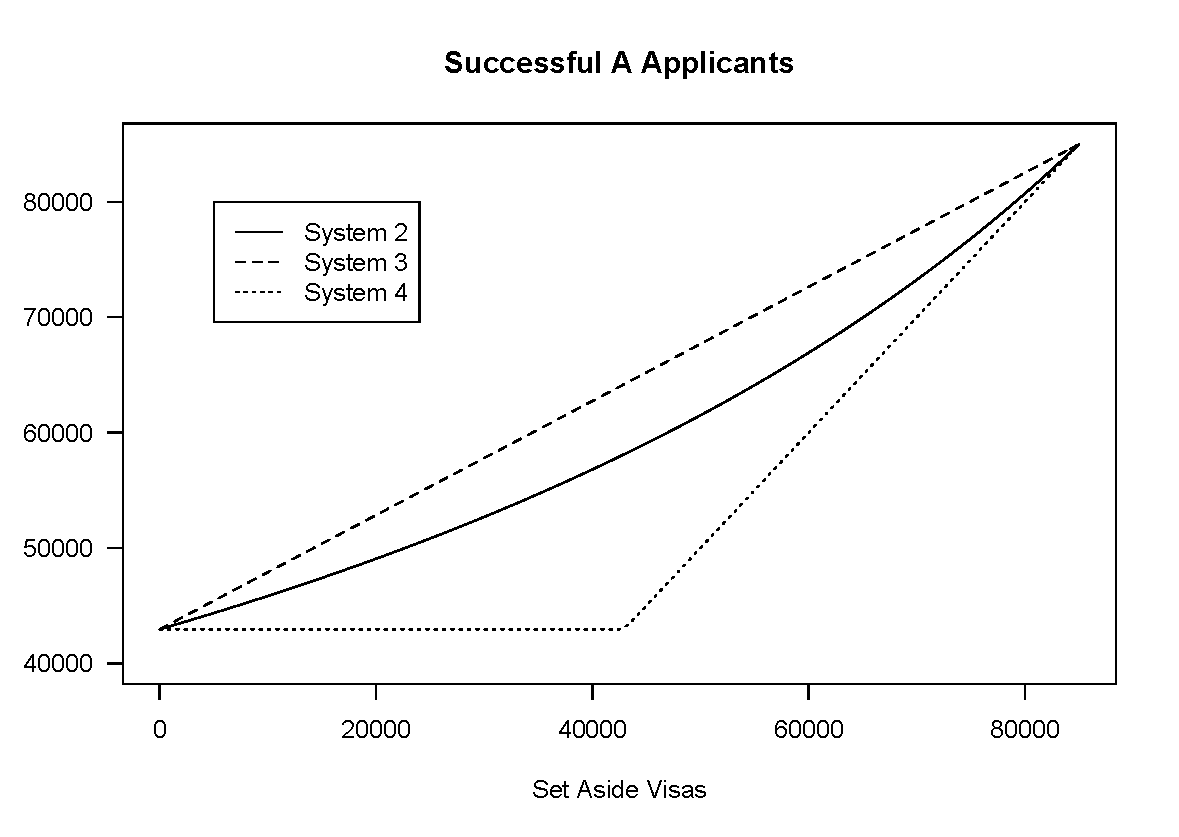
\includegraphics[width = \textwidth]{H1Bplot}
\caption{For any number of set-aside visas (x-axis), implementation details influence the number of visas going to applicants with advanced degrees from US institutions (y-axis).} \label{fig:h1b}
\end{figure}


{\bf Conclusions.} The point that generalizes from this example is that a single set of caps (in this case, 20,000 and 65,000) can have different effects depending on how it is implemented. Whereas a change to the caps might draw a lot of attention, a change to the order in which lotteries are run is likely to slide under the radar. Nevertheless, this change will shift thousands of visas annually to applicants with advanced degrees (and away from those without).



{\bf Parallels to School Choice.} A similar situation arose in the Boston Public School system. In that context, the scarce resource was admission to popular public schools (instead of visas). `A' applicants were those living within walking distance of the school, and `B' applicants were those living farther away. A contentious debate over whether to give priority to students in the walk zone was settled with a compromise: half of seats would be reserved for such students, and half of seats would be open to anybody. This compromise was implemented using System 4 above, which resulted in little -- if any -- advantage for students living in the walk zone. After many years, administrators realized that the nominal set-asides for walk-zone students were having little effect. Rather than changing to Systems 2 or 3 above, the city abolished walk zone priority altogether. For more details, read \link{https://www.dropbox.com/s/mh3rf76ebb8oy3d/Dur-Kominers-Pathak-Sonmez-2017.pdf?dl=0}{this paper.}

%\section{}
%\subsection{}



\end{document}  